\documentclass[]{article}
\usepackage{amsmath}
\usepackage{graphicx}

%opening
\title{Assignment - Constrained optimization\\Interior Point Method applied to linear programming
	problems}
\author{Matteo Bunino}

\begin{document}

\maketitle

\section{Problem definition}
The Predictor-Corrector is an Interior Point Method built to iteratively solve a nonlinear system of equations, obtained by defining the KKT condition for the pair primal-dual problem.\\
The linear system to solve is:
\begin{equation*}
	F(x,\lambda, s) = 
	\begin{bmatrix}
	Ax-b \\[0.3em]
	s+A^T\lambda-c \\[0.3em]
	XSe          
	\end{bmatrix}
	=0
\end{equation*}

According to Newton method for nonlinear system of equation, the system can locally linearized and solved. To linearize this system is necessary to compute the Jacobian of $F$ at each iteration and solve the linear system:
\begin{equation*}
	F'(x_k,\lambda_k, s_k) \cdot 
	\begin{pmatrix}
	\Delta x_k \\[0.3em]
	\Delta \lambda_k \\[0.3em]
	\Delta s_k           
	\end{pmatrix}
	+ F(x_k,\lambda_k, s_k)=0\\
\end{equation*}
\begin{equation*}
\begin{pmatrix}
A & 0 & 0 \\[0.3em]
0 & A^T & I \\[0.3em]
S_k & 0 & X_k           
\end{pmatrix}
\cdot 
\begin{pmatrix}
\Delta x_k \\[0.3em]
\Delta \lambda_k \\[0.3em]
\Delta s_k           
\end{pmatrix}
+ F(x_k,\lambda_k, s_k)=0\\
\end{equation*}
\\
Where $X_k=diag(x_k)$ and $S_k=diag(s_k)$.\\
Interior point methods are variants of Newton method that guarantee that each iterate $(x_k, \lambda_k, s_k)$ satisfy the constraint $x, s\geq0$.
\section{Problem data}
$A=(1, \dots 1)\in \Re^{1*n}$, \\
$b = 1$,\\
$c \in \Re^n:c_i=a$ if $i$ is odd, otherwise 1.\\
$x \in \Re^n$.\\\\
After having built the sparse jacobian of F, using the command spy() it's possible to inspect its structure:

\begin{figure}[h]
	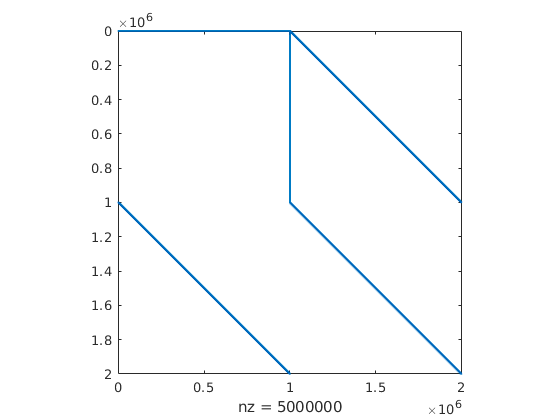
\includegraphics[width=12cm]{code/AA.png}
\end{figure}

Using the command [R,p] = chol(J) it's possible to notice, thanks to the value of p, that the matrix isn't positive definite. Hence I could not use: gradient method, conjugate gradient or Cholesky decomposition.\\
Since this matrix isn't symmetric, I didn't use the LDL decomposition neither.\\\\
Analyzing the structure of the block matrix, I could notice that it's possible to make some reductions, rewriting the left hand part in a more compact way:
\begin{equation*}
\begin{pmatrix}
A & 0 & 0 \\[0.3em]
0 & A^T & I \\[0.3em]
S_k & 0 & X_k           
\end{pmatrix}
\cdot 
\begin{pmatrix}
\Delta x_k \\[0.3em]
\Delta \lambda_k \\[0.3em]
\Delta s_k           
\end{pmatrix}
= 
\begin{pmatrix}
r_a \\[0.3em]
r_b \\[0.3em]
r_c         
\end{pmatrix}
\end{equation*}
Since $X$ is invertible ($x > 0$ is guarateed by the IPM):
\begin{equation*}
	\begin{pmatrix}
	A & 0\\
	-X^{-1}S & A^T
	\end{pmatrix}
	\cdot
	\begin{pmatrix}
	\Delta x_k \\[0.3em]
	\Delta \lambda_k \\[0.3em]
	\end{pmatrix}
	=
	\begin{pmatrix}
	r_a\\
	r_b-X^{-1}r_c
	\end{pmatrix}
\end{equation*}
$S$ is invertible for the same reason:
\begin{equation*}
	\begin{split}
	AS^{-1}XA^T\Delta\lambda&=r_a+AXS^{-1}r_b-AS^{-1}r_c\\
	\Delta s &= r_b-A^T\Delta \lambda\\
	\Delta x &= S^{-1}r_c-XS^{-1}\Delta s\\
	\end{split}
\end{equation*}
The matrix $AS^{-1}XA^T \in \Re^{mxm}$ is a real number, since in this case $m=1$. This makes the computation of the system trivial, avoiding the problem of working with singular or indefinite matrices.
\section{Results}

\begin{figure*}[h]
	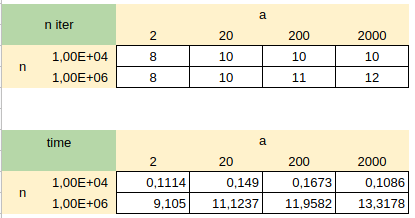
\includegraphics[width=12cm]{table2.png}
	\caption{Starting point of all ones.}
\end{figure*}
\begin{figure}[h]
	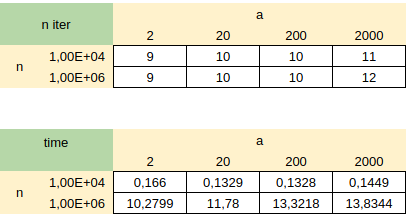
\includegraphics[width=12cm]{table3.png}
	\caption{Starting point of all 100.}
\end{figure}
\begin{figure}[h]
	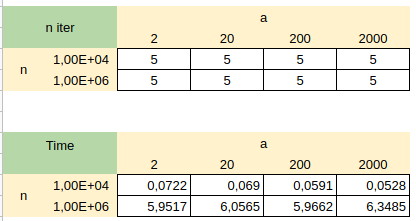
\includegraphics[width=12cm]{table1.png}
	\caption{Starting point as suggested on the book.}
\end{figure}


\end{document}
